\documentclass[dvipdfmx]{jsarticle}
\setcounter{section}{3}
\setcounter{subsection}{3}
\usepackage{xr}
\externaldocument{8.3.1}
\usepackage{amsmath,amsfonts,amssymb,array,comment,mathtools,url,docmute}
\usepackage{longtable,booktabs,dcolumn,tabularx,mathtools,multirow,colortbl,xcolor}
\usepackage[dvipdfmx]{graphics}
\usepackage{bmpsize}
\usepackage{amsthm}
\usepackage{enumitem}
\setlistdepth{20}
\renewlist{itemize}{itemize}{20}
\setlist[itemize]{label=•}
\renewlist{enumerate}{enumerate}{20}
\setlist[enumerate]{label=\arabic*.}
\setcounter{MaxMatrixCols}{20}
\setcounter{tocdepth}{3}
\newcommand{\rotin}{\text{\rotatebox[origin=c]{90}{$\in $}}}
\renewcommand{\thesection}{第\arabic{section}部}
\renewcommand{\thesubsection}{\arabic{section}.\arabic{subsection}}
\renewcommand{\thesubsubsection}{\arabic{section}.\arabic{subsection}.\arabic{subsubsection}}
\everymath{\displaystyle}
\allowdisplaybreaks[4]
\usepackage{vtable}
\theoremstyle{definition}
\newtheorem{thm}{定理}[subsection]
\newtheorem*{thm*}{定理}
\newtheorem{dfn}{定義}[subsection]
\newtheorem*{dfn*}{定義}
\newtheorem{axs}[dfn]{公理}
\newtheorem*{axs*}{公理}
\renewcommand{\headfont}{\bfseries}
\makeatletter
  \renewcommand{\section}{%
    \@startsection{section}{1}{\z@}%
    {\Cvs}{\Cvs}%
    {\normalfont\huge\headfont\raggedright}}
\makeatother
\makeatletter
  \renewcommand{\subsection}{%
    \@startsection{subsection}{2}{\z@}%
    {0.5\Cvs}{0.5\Cvs}%
    {\normalfont\LARGE\headfont\raggedright}}
\makeatother
\makeatletter
  \renewcommand{\subsubsection}{%
    \@startsection{subsubsection}{3}{\z@}%
    {0.4\Cvs}{0.4\Cvs}%
    {\normalfont\Large\headfont\raggedright}}
\makeatother
\makeatletter
\renewenvironment{proof}[1][\proofname]{\par
  \pushQED{\qed}%
  \normalfont \topsep6\p@\@plus6\p@\relax
  \trivlist
  \item\relax
  {
  #1\@addpunct{.}}\hspace\labelsep\ignorespaces
}{%
  \popQED\endtrivlist\@endpefalse
}
\makeatother
\renewcommand{\proofname}{\textbf{証明}}
\usepackage{tikz,graphics}
\usepackage[dvipdfmx]{hyperref}
\usepackage{pxjahyper}
\hypersetup{
 setpagesize=false,
 bookmarks=true,
 bookmarksdepth=tocdepth,
 bookmarksnumbered=true,
 colorlinks=false,
 pdftitle={},
 pdfsubject={},
 pdfauthor={},
 pdfkeywords={}}
\begin{document}
\subsubsection{可微分写像}
\begin{dfn}
$m$次元、$n$次元$C^\infty $級多様体$\left( \mathcal{M},\mathfrak{O} \right) $、$\left( \mathcal{N},\mathfrak{P} \right) $、その多様体$\left( \mathcal{M},\mathfrak{O} \right) $からその多様体$\left( \mathcal{N},\mathfrak{P} \right) $への連続写像$\varphi :\mathcal{M} \rightarrow \mathcal{N} $が与えられたとき、$p\in \mathcal{M}$なる元$\varphi (p)$のその多様体$\left( \mathcal{N},\mathfrak{P} \right) $における近傍$V$で定義された任意の$C^r $級写像$f:V\rightarrow \mathbb{R} $に対し、その写像$\varphi $が連続なので、定理\ref{8.1.3.1}よりその値域$V\left(\varphi^{-1} | V\right)$もその多様体$\left( \mathcal{M},\mathfrak{O} \right) $におけるその元$p$の近傍となる。このときの合成写像$f\circ \varphi : V\left(\varphi^{-1} | V\right) \rightarrow \mathbb{R} $も、その写像たち$\varphi $、$f$が連続なので、連続である。これに加えて、その写像$f\circ \varphi $がその元$p$の近傍で$C^r $級であるとき、その写像$\varphi $はその元$p$で$C^r $級であるといい、$\forall p\in \mathcal{M} $に対し、その元$p$でその写像$\varphi $が$C^r $級であるとき、その写像$\varphi $はその多様体$\left( \mathcal{M},\mathfrak{O} \right) $からその多様体$\left( \mathcal{N},\mathfrak{P} \right) $への$C^r $級写像であるという。特に、その写像$\varphi $がその元$p$で$C^\infty $級である、その多様体$\left( \mathcal{M},\mathfrak{O} \right) $からその多様体$\left( \mathcal{N},\mathfrak{P} \right) $への$C^\infty $級写像であるとき、それぞれその写像$\varphi $がその元$p$で可微分である、その多様体$\left( \mathcal{M},\mathfrak{O} \right) $からその多様体$\left( \mathcal{N},\mathfrak{P} \right) $への可微分写像であるという。
\end{dfn}
\begin{thm}\label{8.3.2.9}
$m$次元、$n$次元$C^\infty $級多様体$\left( \mathcal{M},\mathfrak{O} \right) $、$\left( \mathcal{N},\mathfrak{P} \right) $、その多様体$\left( \mathcal{M},\mathfrak{O} \right) $からその多様体$\left( \mathcal{N},\mathfrak{P} \right) $への連続写像$\varphi :\mathcal{M} \rightarrow \mathcal{N} $が与えられたとき、$\forall p\in \mathcal{M}$に対し、$p\in U$、$\varphi \left(p\right) \in V$、$\chi=\left(\chi_i \right)_{i\in \varLambda_n }$なるそれらの多様体たち$\left(\mathcal{M},\mathfrak{O}\right)$、$\left(\mathcal{N},\mathfrak{P}\right)$におけるある座標近傍系たち$\left(U,\psi\right)$、$\left(V,\chi\right)$を用いて、その写像$\varphi $がその元$p$で$C^r $級であるなら、そのときに限り、$i\in \varLambda_n $なる関数たち$\chi_i \circ \varphi \circ \psi^{-1} $がその元$p$で$C^r $級である。このとき、これらの座標近傍系たち$\left(U,\psi\right)$、$\left(V,\chi\right)$の取り方に依らない。
\end{thm}\par
なお、上の主張での関係は次のように与えられる。
\begin{center}
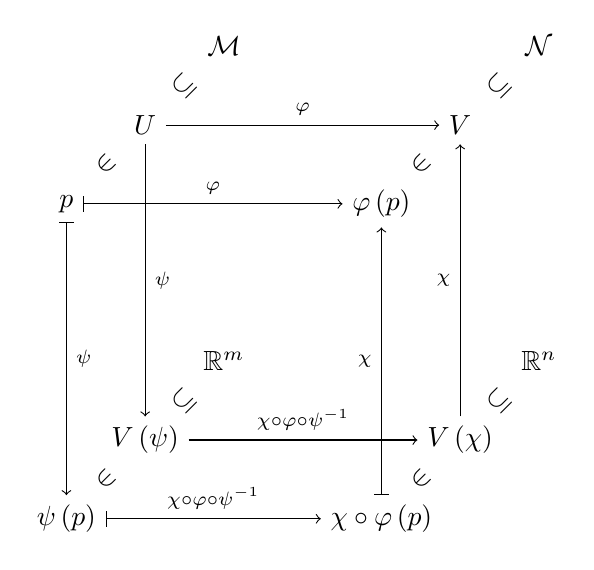
\begin{tikzpicture}[auto]
  \node (a) at (1, 1) {$V\left(\psi\right)$};
  \node (b) at (5, 1) {$V\left(\chi\right)$};
  \node (c) at (1, 5) {$U$};
  \node (d) at (5, 5) {$V$};
  \node (e) at (0, 4) {$p$};
  \node (f) at (4, 4) {$\varphi \left(p\right)$};
  \node (x) at (0.5, 4.5) {\rotatebox{45}{$\in $} };
  \node (x) at (4.5, 4.5) {\rotatebox{45}{$\in $} };
  \node (x) at (1.5, 5.5) {\rotatebox{45}{$\subseteq $} };
  \node (x) at (5.5, 5.5) {\rotatebox{45}{$\subseteq $} };
  \node (x) at (2, 6) {{$\mathcal{M} $} };
  \node (x) at (6, 6) {{$\mathcal{N} $} };
  \node (i) at (0, 0) {$\psi\left(p\right)$};
  \node (j) at (4, 0) {$\chi \circ \varphi \left(p\right)$};
  \node (x) at (0.5, 0.5) {\rotatebox{45}{$\in $} };
  \node (x) at (4.5, 0.5) {\rotatebox{45}{$\in $} };
  \node (x) at (1.5, 1.5) {\rotatebox{45}{$\subseteq $} };
  \node (x) at (5.5, 1.5) {\rotatebox{45}{$\subseteq $} };
  \node (x) at (2, 2) {{$\mathbb{R}^m $} };
  \node (x) at (6, 2) {{$\mathbb{R}^n $} };
  
  \draw [->] (c) to node {$\scriptstyle \varphi $} (d);
  \draw [|->] (e) to node {$\scriptstyle \varphi $} (f);
  \draw [->] (c) to node {$\scriptstyle \psi $} (a);
  \draw [|->] (e) to node {$\scriptstyle \psi $} (i);
  \draw [->] (a) to node {$\scriptstyle \chi \circ \varphi \circ \psi^{-1}$} (b);
  \draw [|->] (i) to node {$\scriptstyle \chi \circ \varphi \circ \psi^{-1}$} (j);
  \draw [->] (b) to node {$\scriptstyle \chi $} (d);
  \draw [|->] (j) to node {$\scriptstyle \chi $} (f);
\end{tikzpicture}
\end{center}
\begin{proof}
$m$次元、$n$次元$C^\infty $級多様体$\left( \mathcal{M},\mathfrak{O} \right) $、$\left( \mathcal{N},\mathfrak{P} \right) $、その多様体$\left( \mathcal{M},\mathfrak{O} \right) $からその多様体$\left( \mathcal{N},\mathfrak{P} \right) $への連続写像$\varphi :\mathcal{M} \rightarrow \mathcal{N} $が与えられたとき、$\forall p\in \mathcal{M}$に対し、$p\in U$、$\varphi \left(p\right) \in V$、$\chi=\left(\chi_i \right)_{i\in \varLambda_n }$なるそれらの多様体たち$\left(\mathcal{M},\mathfrak{O}\right)$、$\left(\mathcal{N},\mathfrak{P}\right)$におけるある座標近傍系たち$\left(U,\psi\right)$、$\left(V,\chi\right)$を用いて、その写像$\varphi $がその元$p$で$C^r $級であるなら、その元$\varphi (p)$のその多様体$\left( \mathcal{N},\mathfrak{P} \right) $における近傍$W$で定義された任意の$C^r $級写像$f:W\rightarrow \mathbb{R} $に対し、その写像$f\circ \varphi $がその元$p$の近傍で$C^r $級となる、即ち、その関数$f\circ \varphi \circ \psi^{-1} $がその元$\psi \left(p\right) $の近傍で$C^r $級となる。特に、定理\ref{8.3.2.1}より$\forall i\in \varLambda_n $に対し、その関数$\chi_i \circ \varphi \circ \psi^{-1} $がその元$\psi \left(p\right) $の近傍で$C^r $級となる。\par
逆に、$i\in \varLambda_n $なる関数たち$\chi_i \circ \varphi \circ \psi^{-1} $がその元$p$で$C^r $級であるなら、その元$\varphi (p)$のその多様体$\left( \mathcal{N},\mathfrak{P} \right) $における近傍$W$で定義された任意の$C^r $級写像$f:W\rightarrow \mathbb{R} $に対し、定義\ref{写像はCs級であることの定義}よりその関数$f\circ \chi^{-1} $もその元$\varphi\left(p\right)$の近傍で$C^r $級であるので、その合成関数$\left( f\circ \chi^{-1} \right) \circ \left( \chi \circ \varphi \circ \psi^{-1} \right) $もその点$\psi^{-1} \left(p\right) $で$C^r $級となる、即ち、その写像$f\circ \varphi $もその元$p$で$C^r $級となる。これはその写像$\varphi $がその元$p$で$C^r $級となることを意味する。\par
このとき、これらの座標近傍系たち$\left(U,\psi\right)$、$\left(V,\chi\right)$とは別に座標近傍系$\left(U',\psi'\right)$、$\left(V',\chi'\right)$をとったとき、仮定よりそれらの合成関数たち$\psi \circ {\psi'}^{-1} $、$\chi' \circ \chi^{-1} $も$C^\infty $級となるので、その合成関数$\left( \chi' \circ \chi^{-1} \right) \circ \left( \chi \circ \varphi \circ \psi^{-1} \right) \circ \left( \psi \circ \psi' \right) $も$C^r $級となる、即ち、その関数$\chi' \circ \varphi \circ \psi' $も$C^r $級となることから、これで示すべきことがすべて示された。
\end{proof}
\begin{dfn}
$m$次元、$n$次元$C^\infty $級多様体$\left( \mathcal{M},\mathfrak{O} \right) $、$\left( \mathcal{N},\mathfrak{P} \right) $、その多様体$\left( \mathcal{M},\mathfrak{O} \right) $からその多様体$\left( \mathcal{N},\mathfrak{P} \right) $への連続写像$\varphi :\mathcal{M} \rightarrow \mathcal{N} $が与えられたとき、  
\end{dfn}
\begin{thebibliography}{50}
\bibitem{1}
  松島与三, 多様体入門, 裳華房, 1965. 第36刷 p24-31 ISBN978-4-7853-1305-0
\bibitem{2}
  松本幸夫, 多様体の基礎, 東京大学出版会, 1988. 第16刷 p37-53 ISBN4-13-062103-3
\bibitem{3}
  新井朝雄, 相対性理論の数理, 日本評論会, 2021. 第1版第1刷 p164-166 ISBN978-4-535-78928-9
\end{thebibliography}
\end{document}
